%!TEX root = ../template.tex
%%%%%%%%%%%%%%%%%%%%%%%%%%%%%%%%%%%%%%%%%%%%%%%%%%%%%%%%%%%%%%%%%%%%
%% chapter2.tex
%% NOVA thesis document file
%%
%% Chapter with the template manual
%%%%%%%%%%%%%%%%%%%%%%%%%%%%%%%%%%%%%%%%%%%%%%%%%%%%%%%%%%%%%%%%%%%%
\chapter{Related Work}
\label{cha:related_work}

% ================
% = Introduction =
% ================
Cloud computing has emerged as an efficient way for modern systems to deal with modern problems, caused by the growth of internet users worldwide over the years \cite{growthInternetUsers}, where scalability became a must and the cloud's ability to offer storage and computing power on demand made it so useful.
With that said, users (including companies) started choosing cloud providers as a convenient way to store their data and services, trusting that data privacy would be assured. However, that is not always the case in modern cloud providers. 

In this chapter, we address existing solutions able to grant a better level of privacy to data, by protecting applications from the \gls{os}/hypervisor regardless of the machine they're running on, increasing the level of trust of users in the remote execution of an application.

These existing solutions are organized in different sections in the following way: 
Section \ref{sec:protect_untrustOS} covers protection against untrusted \gls{os}es; 
Section \ref{sec:tpm_hsm_tees} covers \gls{tee}s and hardware-enabled approaches;
In Section \ref{sec:hardwareTEEs} we cover, in more detail, hardware-enabled \gls{tee} solutions used today;
Section \ref{sec:sgxFrameworks} covers shielded applications and frameworks compatible with Intel-\gls{sgx}, which is the \gls{tee} technology we choose for our approach;
Finally, in Section \ref{sec:summary} we make a critical analysis of the topics previously discussed while covering their main advantages and disadvantages.


% =======================
%  N E W   S E C T I O N        (2.1)
% =======================


\section{Protection in untrusted OSes}
\label{sec:protect_untrustOS}

A lot of applications these days depend on sensitive data to operate. Therefore protecting this data must be taken into account while designing the application. 
One of the things we have to think about is the size of the \gls{tcb}, and how to reduce it as much as possible without losing the operability of the system. 
Typically, the host \gls{os} is considered safe and trustworthy, although that is not always the case. A compromised \gls{os} can give complete access to sensitive data, if not isolated from the application. That’s why this is a major security problem and must be tackled in today’s systems.

Approaches like Virtual Ghost, Flicker, MUSHI, SeCage, InkTag, Sego, all grant security by isolating the sensitive data from the untrusted \gls{os} either by monitoring the application while it runs or by enforcing memory isolation by using virtualization.\newline

%-----------------------------------------
\subsection{Virtual Ghost} 

Virtual Ghost \cite{virtGhostPaper} provides application security against untrusted \gls{os}es by implementing the idea of ghost memory, which is inaccessible for the \gls{os} to read or write, as well as providing trusted services like ghost memory management, key management, and encryption and signing services. 
It relies on sandboxing to protect the system from the \gls{os}, where a thin layer of abstraction is interposed between the kernel and the hardware. This layer works as a library of functions that the kernel can call directly, without needing higher privileges. 
Thus, Virtual Ghost protects the system against a direct threat from the \gls{os}, without losing significant levels of performance.\newline

%-----------------------------------------

\subsection{Flicker} 

Flicker \cite{flickerPaper} provides secured isolated execution of sensitive code by relying on commodity hardware, such as AMD and Intel processors, to run certain pieces of code in a confined environment while reducing the \gls{tcb} to, as few as, 250 additional lines of code. 
When Flicker starts, none of the software already executing can monitor or interfere with its execution and all its traces can be eliminated before non-Flicker execution resumes. 
Thus, with a small TCB and a good level of isolation during the execution phase, where no data is leaked nor possible to access while inside the confined environment, the system can achieve reliability and security.\newline

%-----------------------------------------

\subsection{MUSHI} 

MUSHI \cite{mushiPaper} is designed to deal mainly with multi-level security systems and provides isolation to individual guest \gls{vm}s executing in a cloud infrastructure. MUSHI ensures that \gls{vm}s are instantiated securely and remain that way throughout their life cycle. 
It is capable of offering: (1) \textbf{Trusted Execution}, where both the kernel and user image, as well as MUSHI itself, are attested upon a \gls{vm} start by using a \gls{tpm}, thus defining a trusted initial state; (2) \textbf{Isolation}, where each \gls{vm} executing on the same machine runs isolated, as a way to guarantee confidentiality and integrity; (3) \textbf{User Image Confidentiality}, by encrypting the user image with a cryptographic key provided by the user itself.

MUSHI guarantees confidentiality and integrity of a \gls{vm} even during malicious attacks from both inside and outside the cloud environment.
It trusts a relatively small \gls{tcb}, that includes only the hardware, hardware virtualization, BIOS, and System Management Mode, and can be implemented with quite ease using modern commodity hardware containing SMM memory (SMRAM), necessary for the isolation between the host and \gls{vm}.\newline

%-----------------------------------------

\subsection{SeCage} 

SeCage \cite{SeCagePaper} uses hardware virtualization to protect user-defined secrets from potential threats and malicious \gls{os}es, by isolating sensitive code and critical secrets while denying the hypervisor any possibility of intervention during runtime.
It divides the system into compartments, where secret compartments have all the permissions to access and manipulate the user-defined secrets, and a main compartment responsible for handling the rest of the code.
SeCage is designed to assure the confidentiality of user-secrets, adding a small overhead while supporting large-scale software. To achieve this, it ensures:
\begin{enumerate}
	\item \textbf{Hybrid analysis of secrets}, where static and dynamic analysis are combined to define secret compartments to execute secrets, preventing them from being disclosed during runtime;
	\item \textbf{Hypervisor protection}, using hardware virtualization to isolate each compartment;
	\item \textbf{Separating control and data plane}, where minimal hypervisor intervention is required to deal with communications between compartments. The hypervisor is limited to define policies on whether two compartments can communicate (control plane) for as long as they conform to those policies.\newline
\end{enumerate}


%-----------------------------------------

\subsection{InkTag} 

InkTag \cite{inkTagPaper} also uses a virtualization-based approach in order to grant applications protection from untrusted \gls{os}es.
But unlike SeCage, InkTag admits trust in the hypervisor. The hypervisor is responsible to protect the application
code, data, and control flow from the \gls{os}, allowing applications to execute in isolation, in high-assurance processes (HAP). Trusted applications can communicate directly with the InkTag hypervisor via hypercalls, as a way to detect \gls{os} misbehavior.
It introduces a concept called paraverification, which simplifies the hypervisor by forcing the untrusted \gls{os} to participate in its own verification. As a result, the \gls{os} notifies the InkTag hypervisor upon any update to be made to the state, which the hypervisor can check for correctness. 
InkTag also isolates secure from unsafe data through hardware virtualization and allows each application to specify their own access control policies, managing their data privacy and integrity through encryption and hashing.
Another important aspect of InkTag is recoverability. InkTag hypervisor can protect the integrity of files even if the system crashes, by ensuring consistency between file data and metadata upon a crash.\newline

%-----------------------------------------

\subsection{Sego} 

Similar to InkTag, Sego \cite{segoPaper} is also a hypervisor-based system that gives strong privacy and integrity guarantees to trusted applications. To protect applications from untrusted \gls{os}es, Sego removes the trust from the \gls{os}, relying only on a trusted hypervisor which is assumed to always execute correctly. It also enforces paraverification, where the \gls{os} communicates its intentions to the hypervisor, thus keeping track of its behavior.

\begin{figure}[htbp]
	\centering
	{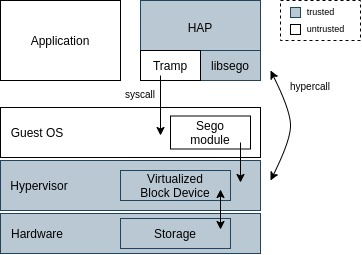
\includegraphics[width=70mm, scale=0.6]{sego}}
	\caption{Sego Architecture Overview}
	\label{fig:segoArchitecture}
\end{figure}

Sego is designed to execute trusted code in a \gls{hap}.
After booting the \gls{os}, the hypervisor starts the \gls{hap}, in a way that the \gls{hap} itself can verify its own initial code and data, similar to a \gls{tpm}.
Once running, the hypervisor ensures that the \gls{hap}’s registers and trusted address space are isolated from the \gls{os}. Every time the \gls{hap} wants to perform a system call, it must inform
the hypervisor of its intent so that the hypervisor can verify the \gls{os}'s activity. \gls{hap}s use a
small library called libsego as a way to handle system calls and get Sego services without having to change their code. Each \gls{hap} also contains an untrusted trampoline code, that
uses to interact with the \gls{os}. This protects its control-flow, since it uses this trampoline as the issuer for system calls, therefore never compromising the \gls{hap} itself. Figure \ref{fig:segoArchitecture} shows well enough Sego’s overall design without going into too much dept, indicating which components are included in the \gls{tcb} and which are not.
Context switches are handled by the hypervisor, thus hiding any information about the \gls{hap} from the \gls{os}.
Sego does not guarantee \gls{os} availability. A compromised \gls{os} can simply shut down or refuse to schedule processes. However, this is easily detected.

In conclusion, although all these approaches are prepared to isolate an application from untrusted hosts, they emphasize the use of software to do it, leaving behind the importance of hardware trustworthiness to the whole system.

In the following sections, we will take a look at existing solutions that are able to tackle also hardware related security problems.
% =======================
%  N E W   S E C T I O N        (2.2)
% =======================

\section{Hardware-Enabled TEE - Trusted Execution Environments}
\label{sec:tpm_hsm_tees}

A \gls{tee} is an abstraction provided by both software and hardware that guarantees isolated execution of programs in a machine from the host \gls{os}, hypervisor, or even system administrators, preventing them from leveraging their privileges. A \gls{tee} also provides integrity of applications running inside it, along with the confidentiality of their assets.
The first attempts to implement a \gls{tee} on a cloud system consisted of combining a hypervisor with isolation properties and a \gls{tpm}. 

A \gls{tpm} \cite{tpmPaper} consists of a hardware chip, called microcontroller, that aims to create a trustable platform through encryption and authenticated boot, and make sure it remains trustworthy through remote attestation. 
It provides cryptographic functions that can't be modified, and a private key (Endorsement Key) that is unique to every \gls{tpm} made, working as an identifier for the \gls{tpm} itself.
However, \gls{tpm}s have several problems when applied to cloud systems, due to being designed with the intention to offer security to a single machine. It is not flexible enough to guarantee that anyone can get the encrypted data from a different node.
Thus, a distributed environment would not be the best kind of environment for a \gls{tpm} to work on.

The current best practice for protecting secrets in  cloud systems uses \gls{hsm}s. 
An \gls{hsm} \cite{hsmPaper} is a physical hardware component that provides and stores cryptographic keys used to encrypt/decrypt data inside a system. \gls{hsm}s also perform cryptographic operations (e.g. encryption, hashing, etc.) as well as authentication through verifying digital signatures and accelerating \gls{ssl} connections \cite{hsmThesis}, by relieving the servers from some of the workload caused by operations involving cryptography. 
Thus, the system can protect critical secrets (cryptographic keys) and support a range of cryptographic functions.

With that in mind, new hardware-enabled solutions were developed to be more flexible and cloud-friendly than the \gls{tpm} or to incorporate the advantages of \gls{hsm} to the system. We'll dive into technologies like ARM TrustZone, Intel SGX, AMD-SEV, and some others, in the following section.


% =======================
%  N E W   S E C T I O N        (2.3)
% =======================


\section{Hardware-Enabled TEE Solutions}
\label{sec:hardwareTEEs}

The idea of using hardware to provide trusted execution environments to run code appeared as a way to deal with piracy, with examples like TCPA \cite{tcpaPaper} and Microsoft's Palladium \cite{microsoftPalladium} being the most popular at that time. By providing protection during execution through hardware, it became possible to encrypt data (e.g. DVD's) that could only be decrypted by specific hardware, making it almost impossible to pirate. 
Although these approaches were effective back in the day, both of them place their trust in the hardware, not trusting the \gls{os} entirely. 
Thus, since any application does not trust the \gls{os}, it does not trust the application to properly use its resources either. Therefore, some of the protection aspects of the \gls{os} should be moved into the hardware, while also changing the interface between the \gls{os} and the application so it supports hardware security features. 

\gls{xom}, described in the next subsection, was one of the first approaches developed as a way to deal with these changes, and one of the stepping stones that lead us to the modern \gls{tee} technology we see nowadays, that we will also describe in this section.

\subsection{XOM}
\label{ssec:xom}

\gls{xom} \cite{xomPaper} is a processor architecture able to provide copy protection and tamper-resistance functions, 
useful for enabling code to run in untrusted platforms, deployment of trusted clients in distributed systems like banking transactions, online gaming, electronic voting, but also fundamental to deal with piracy back in the day it was published. 

The main idea is to only trust the processor to protect the code and data, thus not trusting the main memory nor any software, including the host \gls{os}.
However, this idea of only trusting hardware has some implications for \gls{os}es design. This happens due to the fact that sharing hardware resources between multiple users is a hard job, especially without trusting any software. It is usually easier to have these policies performed by the \gls{os}. Therefore, not trusting the software entirely can sometimes be a drawback.  
For \gls{xom} architecture to be used, it is required a specific \gls{os} (XOMOS). XOMOS runs on hardware that supports tamper-resistant software and is adapted to manage hardware resources for applications that do not trust it.
\gls{xom} offers protection against attackers who may have physical access to the hardware itself, as well as main memory protection if compromised. For it, the XOM processor encrypts the values in memory and stores the hash of those values in memory as well. It then only accepts encrypted values from memory if followed by a valid respective hash. 



\subsection{ARM TrustZone}
\label{ssec:armtz}

ARM TrustZone \cite{armTZPaper} is ARMs approach to offer a \gls{tee} where software can execute in a secured and trustable way, safe from the host machine, as well as its \gls{os} and/or hypervisor. 

To create this abstraction, ARM processors implement two virtual processors backed by hardware access control, where the software stack can switch between two states: secure world (SW) and normal world (NW). 
The first one has higher privileges than the second one, therefore it can access NWs copies of registers, but not the other way around. SW is also responsible for protecting running processes in the \gls{cpu} while providing secure access to peripherals. 
Each world acts as a runtime environment and has its own set of resources. These resources can be partitioned between the two worlds or just assigned to one of them, depending on the ARM chip specs.
For the context switch between worlds, ARM processors implement a secured mode called Secure Monitor, where there is a special register responsible of determine if the processor runs code in SW or NW. 
Most ARM processors also offer memory curtaining. This consists of the Secure Monitor allocating physical addresses of memory specifically to the SW, making this region of memory inaccessible to the rest of the system.
By default, the system boots always in SW so it can provision the runtime environment before any untrusted code start to run. It eventually transitions to NW where untrusted code can start to be executed. 

\subsection{AMD-SEV}
\label{ssec:amdsev}
AMD Secure Encrypted Virtualization (SEV) \cite{amdPaper} is the AMD approach to provide a \gls{tee}, integrated with virtualization. It is a technology focused on cloud computing environments, specifically in public \gls{iaas}, as its main goal is to reduce trust from higher priviledged parties (\gls{vmm}s or \gls{os}) so that they can not influence the execution on the other "smaller" parties (\gls{vm}s). 
To achieve this, AMD grants encryption of memory through a technology called Secure Memory Encryption (SME), or through TransparentSME (TSME) if the system runs a legacy \gls{os} or hypervisor with no need for any software modifications.
After the data is encrypted, SEV integrates it with AMD virtualization architecture to support encrypted \gls{vm}s. By doing this, every \gls{vm} is protected from his own hypervisor (\gls{vmm}), disabling its access to the decrypted data. Although incapable of accessing the \gls{vm}, the \gls{vmm} is still responsible for controlling each \gls{vm}'s resources. 
Thus, AMD provides confidentiality of data by removing trust from the \gls{vmm}, creating an isolated environment for the \gls{vm} to run, where only the \gls{vm} and the processor can be trusted. 

However, ADM-SEV does not provide integrity of data, allowing replaying attacks to take place, and has a considerably large \gls{tcb}, since the \gls{os} of each \gls{vm} is trusted \cite{amdSEVPaper}. 

\subsection{Sanctum}
\label{ssec:sanctum}
Sanctum \cite{sanctumPaper} offers strong isolation of software modules, although following a different approach focused on avoiding unnecessary complexity.
To make this possible, Sanctum, which typically runs in a RISC-V processor, combines minimal invasive hardware modifications with a trusted software security monitor that is receptive to analysis and does not perform cryptographic operations using keys. 
This minimality idea consists of reusing and slightly modifying existing well-understood mechanisms, while not modifiying \gls{cpu} building blocks, only adding hardware to the interfaces between blocks. This causes Sanctum to be adaptable to many other processors besides RISC-V.

Sanctum is a practical approach that shows that strong software isolation is achievable with a small set of minimally invasive hardware changes, causing reasonably low overhead. 
This approach provides strong security guarantees dealing with side-channel attacks, such as cache timing and passive address translation attacks.

\subsection{Intel-SGX}
\label{ssec:intelsgx}

Intel Software Security Guard Extensions (SGX) \cite{intelSGX} are a set of instructions built-in Intel \gls{cpu}s, that allows programmers to create \gls{tee}s, by using enclaves. Enclaves are isolation containers that create a trusted environment where sensitive code can be stored and executed inside, ensuring integrity and confidentiality to it. By doing so, it reduces the \gls{tcb} in a way that most of the system software, apart from the enclaves and the \gls{cpu}, is considered not trusted.

A system that incorporates \gls{sgx} under its architecture is divided into two: a trusted component being the enclave, and an untrusted component being the rest of the system.
Enclaves are mapped into private regions of memory - called the enclave page cache (EPC) - where only the \gls{cpu} has access to, where code running outside the enclave cannot access the enclave memory region, but code running inside can access untrusted memory. This is made possible by a list of functions incorporated.
Enclaves are initiated by untrusted code, using the ECREATE function, which initializes the EPC in memory. One of the downsides of SGX consists of the fact that the size of EPCs depends on the hardware used in the system, and it's usually quite limited. This can imply that a larger application can't fit entirely into the EPC. To deal with this, SGX provides a mechanism for swapping pages between the EPC and the untrusted memory. But since this process involves a lot of encryption and decryption operations to keep the integrity of data, it can be a problem performance-wise. 

\begin{figure}[htbp]
	\centering
	{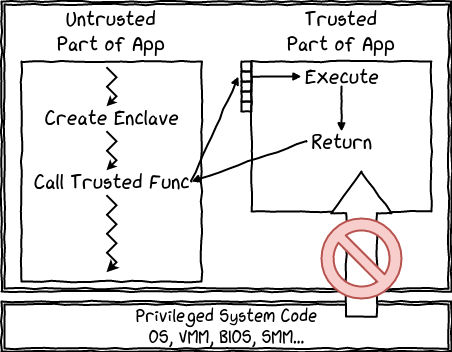
\includegraphics[width=80mm, scale=0.8]{intelsgx_enclave2}}
	\caption{Intel-SGX Enclave execution flow}
	\label{fig:sgxEnclave}
\end{figure}

Although the main purpose of SGX is to isolate the application, even from the host \gls{os}, there are other instructions to interact with the flow of the enclave, that an application can use to deal with the lack of utility libraries, that are often offered by the \gls{os} itself.
EENTER and EEXIT are examples used for a thread to enter and leave the enclave, by switching the CPU enclave mode. This allows a thread, for example, to make calls for privileged instructions, which isn't possible while inside the enclave, and re-enter it after, with safety measures assured by the SGX. The fact that when executing enclave code the system can't run privileged instructions, makes that the threads need to exit and re-enter the enclave to execute them. Such transitions come at a cost since a lot of security measures take place (checks and updates) to ensure that the integrity of the code running inside the enclave is kept intact. This may involve a lot of page swapping between the EPC and untrusted memory which, as we stated before, takes a lot of effort from the system.
ECALLS and OCALLS are another examples of instructions, that are used as a way to securely communicate between trusted and untrusted parties. 


% =======================
%  N E W   S E C T I O N        (2.4)
% =======================


\section{SGX-Enabled Frameworks and Shielded Applications}
\label{sec:sgxFrameworks}
The need for cloud computing is constantly growing in modern applications, based on the fact that it is a cost-effective and practical solution to run large distributed applications. However, the fact that it requires users to fully trust the cloud provider with their code and data creates some trust concerns for developers.
Although the usage of \gls{tee}s like \gls{sgx} aims to tackle this problem by running and storing sensitive data in an isolated environment, protecting that data from unauthorized access, \gls{sgx} itself has some limitations and does offer this extra level of security at some costs for the systems. 

Hence, to deal with the \gls{sgx} limitations, some approaches were developed to be implemented on top of it, as a way to make systems more practical by the integration of trusted computation. 
We will discuss those approaches in the next subsections.



\subsection{Shielded protected applications in untrusted Clouds}
\label{ssec:shieldedApps}

As we said previously, cloud computing is becoming more and more adopted in today's systems. 
By being such a popular technology, it is a must that their users' data remains confidential. 
However, most of today's cloud systems are build using a classical hierarchical security model more worried about the cloud providers' software itself then their users' code. 
Hereupon, for the users of a cloud platform to trust the provider software entirely, as well as the provider staff (i.e. system administrators or anyone with physical access to the hardware), some new measures need to be adapted.

Several approaches were developed as a way to give the user some sense of privacy, by creating the notion of shielded execution for applications running in the cloud. 
This concept consists of running server applications in the cloud inside of an isolated compartment. The cloud provider is limited to offer only raw resources (computing power, storage, and networking) to the compartment, without being able to access any of the  data, except the one being transmitted over the network. 
Assuring a shielded execution of an application fundamentally means that both confidentiality and integrity are granted and that if the application executes, it behaves as it is expected. As for the provider, it retains control of the resources and may protect itself from a malicious guest \cite{havenPaper}. 


\subsection{SCONE}
\label{ssec:scone}

Container-based virtualization has become quite popular for offering better performance properties than the use of \gls{vm}s, although it offers weaker isolation guarantees, and therefore less security. 
That's why we observe that containers usually execute network services (i.e. REDIS). These are systems that don't need as many system calls as others since they can do a lot via networking, thus keeping a small \gls{tcb} for increased security.

SCONE \cite{sconePaper} is a mechanism for Linux containers that increases the confidentiality and integrity of services running inside them by making use of Intel-\gls{sgx}.
SCONE increases the security of the system while keeping the performance levels reasonable. 
It does it by: 

(1) reducing as much as possible the container's \gls{tcb}, by linking a (small) library inside the enclave to a standard C library interface exposed to container processes. System calls are executed outside the enclave, and networking is protected by \gls{tls};

(2) maximizes the time threads spend inside the enclave by supporting user-level threading and asynchronous system calls, thus allowing a thread outside the enclave to execute system calls without the need for enclave threads to exit.
This increases the performance since major performance losses are caused by enclave threads entering/exiting, due to the costs of encrypting/decrypting the data.


\begin{figure}[htbp]
	\centering
	{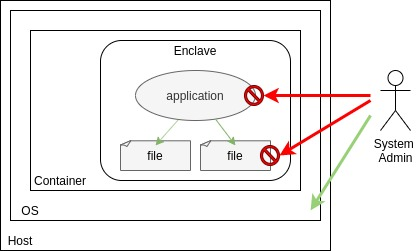
\includegraphics[width=80mm, scale=0.8]{sconeEnclave}}
	\caption{Scone Protection for SGX Enclaves}
	\label{fig:sconeEnclave}
\end{figure}


SCONE also has a mechanism for remote attestation, in which a remote component can attest applications running inside SCONE containers, as a way to check their integrity and to make sure they run as they were instructed to.

\subsection{Haven}
\label{ssec:haven}

Haven is the first system to achieve shielded execution of unmodified legacy applications for a commodity \gls{os} (Windows) and hardware, achieving mutual distrust with the host software.
It leverages Intel-\gls{sgx} to protect against privileged code and physical attacks, but also against the challenge of executing unmodified legacy binaries while protecting them from an untrusted host.
Instead of shielding only specific parts of applications and data by placing them inside enclaves, Haven aims to protect entire unmodified applications, written without any knowledge of \gls{sgx}. 
However, executing entire chunks of legacy binary code inside an \gls{sgx} enclave pushes the limits of the \gls{sgx} itself, and while the code to be protected was written assuming that the \gls{os} executing the code would run it properly, this may not be the case since the \gls{os} can be malicious. For this latest problem, the so-called Iago attack \cite{iagoAttacks}, Haven uses a library \gls{os} adapted from Drawbridge \cite{drawbridge} running inside an \gls{sgx} enclave. 
By combining it with a remote attestation mechanism, Haven is able to guarantee to the user end-to-end security without the need of trusting the provider.
Although this approach may need a substantial \gls{tcb} size (LibOS quite large), all this code is inside the enclave, which makes it under users' control. 

That's the main goal of Haven: give the user trust by granting confidentiality and integrity of their data when moving an application from a private area to a public cloud. 


\subsection{OpenSGX}
\label{ssec:openSGX}

OpenSGX \cite{opensgx_paper} was developed as a way to help with access to \gls{tee} software technologies, since this type of technologies were only available for a selected group of researchers. 
It was made available as an open-source platform, and by providing \gls{tee} and \gls{os} emulation, it contributed a lot for expanding the possibility of research in this area, as well as promoting the development of SGX applications. 
OpenSGX emulates the hardware components of Intel-SGX and its ecosystem, including \gls{os} interfaces and user libraries, as a way to run enclave programs. To emulate Intel-\gls{sgx} at instruction-level, OpenSGX extended an open-source emulator, QEMU.

Its practical properties result from six components working together: 
(1) \textbf{Hardware emulation module}: \gls{sgx} emulation, by providing \gls{sgx} instructions, data structures, \gls{epc} and its access protection, as well as \gls{sgx}' processor key; 
(2) \textbf{\gls{os} emulation}: since some \gls{sgx} instructions are privileged (should be executed by the kernel), OpenSGX defines new system calls to perform \gls{sgx} operations, such as dynamic memory allocation and enclave provisioning; 
(3) \textbf{Enclave loader}: enclave must be properly loaded to \gls{epc}; 
(4) \textbf{User library}: provides a library (sgxlib) with a useful set of functions to be used inside and outside the enclave; 
(5) \textbf{Debugging support}; 
(6) \textbf{Performance monitoring}: allow users to collect performance statistics about enclave programs.

\begin{figure}[htbp]
	\centering
	{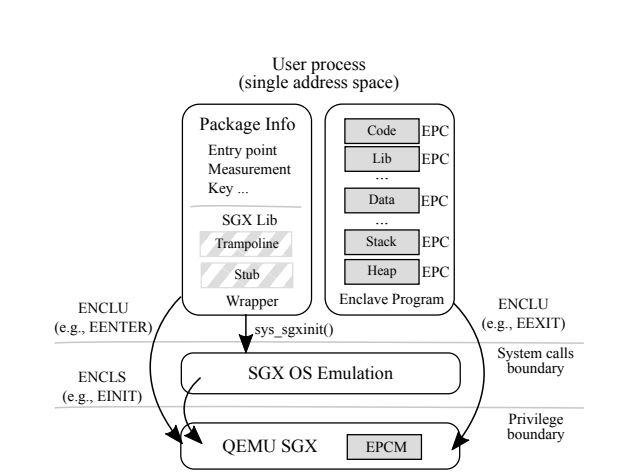
\includegraphics[width=0.7\linewidth]{opensgx_design}}
	\caption{Overview design of OpenSGX framework and memory state. Source: \cite{opensgx_paper}}
	\label{fig:openSGXDesign}
\end{figure}

In Figure \ref{fig:openSGXDesign} we see an illustration of this framework, where a regular program (Wrapper) and a secured program (Enclave Program) both run as a single process in the same virtual address space. Since Intel-\gls{sgx} uses privilege instructions to setup enclaves, the requests from the Wrapper program are handled by the OpenSGX set of system calls.
OpenSGX was proven capable of running non-trivial applications while promoting the implementation and evaluation of new ideas. By being the first open-source framework to emulate an \gls{sgx} environment, it was  fundamental to the growth of the \gls{tee} field.


\subsection{Panoply}
\label{ssec:panoply}

Panoply \cite{panoplyPaper} is a system that works as a bridge between \gls{sgx}-native abstractions and standard \gls{os} abstractions, required by most commodity Linux applications. 
It divides a system into multiple components, called micro-containers (or "micron"), and runs each one of them inside its own enclave. 
However, when microns communicate with each other, their communication goes through a channel under \gls{os} control. Thus, Panoply design goals are focused on supporting \gls{os} abstractions with a low \gls{tcb}, while also securing inter-enclave communications.

Panoply's design consists of a set of runtime libraries (shim library included) and a build toolchain that helps developers to prepare microns.
With this, a programmer can assign annotations to functions as a way to specify which micron should execute a specific function. If not assigned any annotation, a function will be designated to a default micron, who shall execute it. Inter-micron flow integrity is also provided during this stage. 
Each micron is given a micron-id when it starts, which will be used for all further interactions with other microns. It will use this id as a way to assure that only authorized microns can send/receive messages.
To extend this inter-micron interaction security, Panoply also provides authenticated encryption of every message, makes use of unique sequence numbers, and acknowledgment messages are sent for every inter-enclave communication, thus protecting the containers from silent aborts, replaying, or tampering attacks.

Unlike many other \gls{sgx}-based frameworks, Panoply supports unlimited multi-threading and forking. Multi-threading in a way that, if a micron reaches its maximum concurrent thread limit, a new micron is launched and all shared memory operations are safely performed. Forking is achieved by replicating a parent micron's data and sending it to the child, over a secure communication. 


\subsection{VC3}
\label{ssec:vc3_mapreduce}

Verifiable Confidential Cloud Computing (VC3) \cite{vc3Paper} is a framework that achieves confidentiality and integrity of data, as well as verifiability of code execution with good performance through MapReduce \cite{mapReduce} techniques. It uses Intel SGX processors as a building block and runs on unmodified Hadoop \cite{hadoop}.
In VC3 users implement MapReduce jobs, compile and encrypt them, thus obtaining a private enclave code, named \textbf{E-}. They then join it with a small portion of public code called \textbf{E+}, which implements the protocols for key exchange and job execution.
Users then upload the resulting binary code to the cloud, where enclaves containing both E- and E+ are initialized by an untrusted framework F. 

\begin{figure}[tbp]
	\centering
	{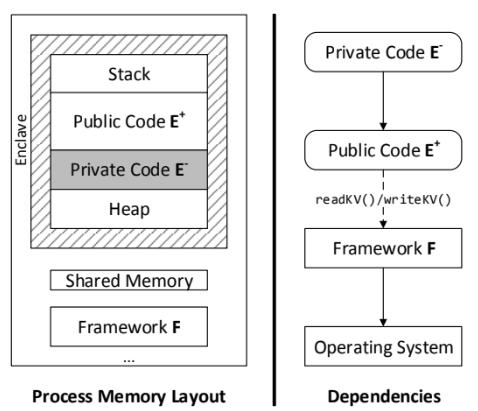
\includegraphics[width=60mm, scale=0.6]{vc3_design}}
	\caption{VC3 memory design model and component dependencies. Source: \cite{vc3Paper}}
\end{figure}

A MapReduce begins with a key exchange between the user and the \textbf{E+} code running in the enclave. After this, \textbf{E+} can proceed to decrypt \textbf{E-} and process the encrypted data. VC3 isolates this processing from the \gls{os} by keeping an interface between the E+ layer and the outside of the enclave. This interface consists of basically two functions: \textbf{readKV()} and \textbf{writeKV()}, for reading or writing a key-value pair on Hadoop, respectively. Also, the data inside the enclave is passed to the outside, more specifically from \textbf{E+} to the untrusted F, by using a virtual address space shared by both.
With VC3, both \textbf{E-} and the user data are always encrypted while in the cloud, except when processed by the trusted processor, while allowing Hadoop to manage the execution of VC3 jobs. Map and reduce nodes are seen as regular worker nodes to Hadoop, therefore Hadoop can keep providing its normal scheduling and fault-tolerance mechanisms, as well as load balancing. VC3 considers Hadoop, as well as both the \gls{os} and the hypervisor as untrusted, thus keeping the \gls{tcb} size as small as possible.

\subsection{Trusted ZooKeeper Approach}
\label{ssec:protected_zookeeper}

ZooKeeper \cite{zookeeper} is a replicated synchronization service for distributed systems with eventual consistency that does not guarantee the privacy of stored data by default. 

Trusted ZooKeeper was presented in \cite{protectedZooKeeper} as an approach that eliminates these privacy concerns, by placing an additional layer between the client and the ZooKeeper, referred to as ZooKeeper Privacy Proxy (ZPP). ZPP is the layer responsible for the encryption of all sensitive information, during a communication between a client and the ZooKeeper. 
Clients communicate with the proxy via SSL, where the packets are encrypted by an individual session key. Here, ZPP acts like a normal ZooKeeper replica to the client. 
After receiving the packets from the client, ZPP extracts the sensitive data, encrypts it with a mechanism that allows the data to be decrypted by the proxy later on, and forwards the encrypted packet to a ZooKeeper replica where it can be stored with integrity ensured.
ZPP runs inside a \gls{tee}, located in the cloud, allowing it to store encryption keys and process data safely. As a result, even if the threat comes from the cloud provider itself, the integrity of the data will still be granted since the attacker won't be able to access or alter anything running inside the \gls{tee}.
ZPP also retains all original ZooKeeper functionality and does not affect ZooKeeper's internal behavior. Therefore adapting existing ZooKeeper applications to this concept can be done with quite ease.

This approach allows applications in the cloud to use ZooKeeper without privacy concerns at the cost of a small decrease in throughput.

\subsection{Ryoan}
\label{ssec:ryoan_sandboxing}

Ryoan \cite{ryoanPaper} consists of a distributed sandbox approach that allows users to protect the execution of their data. This is achieved with the help of Intel-\gls{sgx} \cite{intelSGX} \cite{sgxPaper} technology, by running NaCl (Google Native Client) sandbox instances inside enclaves, protecting the data from untrusted software while also preventing leaks of data, which is a weakness of enclaves caused by side-channel attacks.
Ryoan does not include any privileged software (e.g. OS and hypervisor) in its \gls{tcb}. It trusts only the hardware (\gls{sgx} enclaves) to assure the secrecy and integrity of the data.

Its main goal is to prevent leakage of secret data. This is done by keeping the modules from sending sensitive data over communications outside the system boundaries, but also by eliminating the possibility to store data into unprotected memory regions, as well as crossing off the possibility to make most system calls, granted by using NaCl instances. 
Ryoan's approach consists of confining the untrusted application in a NaCl instance, responsible for controlling system calls, I/O channels, and data sizes. This NaCl sandbox is running inside enclaves' memory region and can communicate with other NaCl instances, forming a distributed sandbox between users and different service providers. Inside the sandbox, the untrusted application can execute safely on secret data. The NaCl sandbox uses a load time code to ensure that the module cannot do anything it shouldn't, thus preventing it from violating the sandbox. To handle faults, exceptions, or errors inside the NaCl sandbox, Ryoan uses an unprotected trampoline code, that can enter the enclave and read the information about the fault, so it can handle it.
\subsection{Opaque}
\label{ssec:opaque}

Opaque \cite{opaquePaper} is a distributed data analytics platform that guarantees encryption, secure computation, and integrity to a wide range of queries. Therefore, instead of being implemented in the application layer or the execution layer as this kind of security approaches usually are, Opaque is implemented in the query optimization layer. 

It is implemented with minimal modifications on Apache Spark \cite{apacheSparkPaper}, a framework for data processing and analytics, and leverages Intel-\gls{sgx} technology as a way to grant confidentiality and integrity of the data. 
However, the use of enclaves can still be threatened by access pattern leakage that can occur at memory-level, when a malicious OS infers information about encrypted data just by monitoring memory page accesses, and also at network-level when network traffic reveals information about encrypted data.
Opaque hides access patterns in the system by using distributed oblivious relational operators and optimizes these by implementing new query planning techniques. It can be executed in three modes: 
(1) \textbf{Encryption mode} - provides data encryption and authentication, while granting correct execution;
(2) \textbf{Oblivious mode} - provides oblivious execution, protecting against access pattern leakage;
(3) \textbf{Oblivious pad mode} - extends the oblivious mode by adding prevention of size leakage.


\subsection{Graphene-SGX}
\label{ssec:grapheneSGX}

The usage of Intel-\gls{sgx} and similar technologies have proven to add a great sense of privacy to the storage and execution of data. However, these technologies impose restrictions (e.g., disallowing system calls inside the enclave) that require the applications to be  adapted to this technology, so they can benefit from their properties. 

Graphene-SGX \cite{graphenePaper} came to help circumvent these restrictions, while still assuring security to the data. It is a libraryOS that aims to reproduce system calls so that unmodified applications can use them to keep executing normally without interacting directly with the OS or hypervisor. 
By using a libraryOS, the system is expected to lose performance and, since a new layer of software was added, increase the size of the TCB. 
Although these assumptions are true, they are quite often exaggerated. Graphene-SGX's performance goes from matching a Linux process to less than 2x, in most executions of single-processes.
Graphene-SGX has also shown some great results comparing it to other similar approaches that use shim layers, such as SCONE \cite{sconePaper} and Panoply \cite{panoplyPaper}, where it shows to be performance-wise similar to SCONE and faster 5-10 percent than Panoply, while adding 54k lines of code to the TCB comparing to SCONE's 97k and Panoply 20k.

Graphene's main goal is to run unmodified applications on \gls{sgx} quickly. Thus, whilst the size of the \gls{tcb} is not the smallest comparing to the other approaches, developers can reduce the \gls{tcb} as needed, as a way to reach a more optimal solution. 
Graphene-SGX also supports application partitioning, enabling it to run small pieces of one application in multiple enclaves. This can be useful, for instance, to applications with different privilege levels, while still increasing the security of the application.


\subsection{Other approaches}
\label{ssec:otherSGXFrameworks}

Other approaches appeared as a way to deal with more specific problems, by making use of trusted computing. We'll go into topics like SGX-Enabled Networking, Administration of Cloud Systems, Virtualization, Containers, searchable Encryption as well as encrypted Databases, and how to take the best advantages of \gls{sgx} in these specific areas. \newline


%-----------------------------------------
\textbf{SGX-Enabled Network Protocols and Services.} 
The increased need for security seen nowadays caused network-related technologies to become popular, from security protocols (\gls{tls}) to anonymous browsers (Tor), leading to a lot of effort by the community to make viable approaches to tackle network security problems. 
Hardware approaches capable of providing \gls{tee}s (e.g. Intel-\gls{sgx}) are some of those contributions, which deal with modern network security concerns as a way to, for example, solve policy privacy issues in inter-domain routing, thus protecting ISPs policies.
In \cite{torSGXPaper} it is shown that leveraging hardware protection of \gls{tee}s can grant benefits, such as simplify the overall design of the application, as well as securely introduce in-network functionality into \gls{tls} sessions. The same paper also presents a possible approach to reach security and privacy on a network level, by building a prototype on top of OpenSGX, that shows that \gls{sgx}-enabled applications have modest performance losses compared to one with no \gls{sgx} support, while significantly improving its security and privacy.

Also at the networking security level, the adoption of Network Function Virtualization (NFV) architecture by applications nowadays implies the creation of an internal state as a way to allow complex cross-packet and cross-flow analysis. 
These states contain sensitive information, like IP addresses, user details, and cached content (e.g. profile pictures), creating the necessity to ensure their protection from potential threats.
S-NFV \cite{sNFVPaper} has proven to be a valid approach, by providing a secure framework for NFV applications, securing NFV states by using Intel-\gls{sgx}.
S-NFV divides the NFV application into two: S-NFV enclave and S-NFV host. The enclave is responsible to store the states and state processing code, while the host deals with the rest.
In \cite{sNFVPaper} by implementing the S-NFV approach with Snort \cite{snortPaper} on top of OpenSGX was
concluded that this \gls{sgx}-enabled approach results in bigger overheads (approx. 11x for
gets and 9x for sets) than an \gls{sgx}-disabled Snort application, at the cost of extra security.\newline

%-----------------------------------------
\textbf{Trusted Cloud-Based System Administration.}
The usage of cloud platforms leads to a significant increase in security and privacy risks. Thus, cloud services are now highly dependent on trusting their administrators, as well as their good behavior. Since this is not always the case, it has become a must to protect the users from potential cloud system administration threats. 
To tackle this problem, some solutions have been proposed with the help of trusted computing technology. However, their focus has been conducted on Infrastructure-as-a-Service (IaaS) environments, which are simpler to maintain than in PaaS and SaaS approaches.

\cite{sgxCloudThesis} proposes a solution that addresses trustworthiness and security in PaaS and SaaS environments, while preserving essential system administration functions by leveraging Intel-\gls{sgx}. Thus, this solution provides an environment for cloud customers to review the security conditions of cloud nodes, more specifically those that run their applications and handle their data.
The main idea behind this approach is to allow the administrative staff necessary privileges according to escalation policies enforced for different roles, instead of never granting full administrative privileges on the computing nodes.
The administrative roles for cloud nodes are divided into four or five independent roles, depending if it is a SaaS or PaaS environment, each with their own permissions. Each role works under the supervision of internal or external auditors. The internal auditors being the ones hired by the provider, while the external are hired by customers, as a way to execute protocols decided by both in a trustable way. The solution enables control of cloud trusted nodes operational states, designated to run customer's computations, as well as remote attestation of the boot sequence of PaaS or SaaS stacks. Finally, by including logging of changes in node's states, this solution is able to offer trustworthy execution of functions and protocols.
The approach was shown in \cite{sgxCloudThesis} to have a minimal performance impact, as well as low storage overheads while proving to be a compelling approach that can be used to increase the detail of management protocols and tools in cloud environments and data-centers.\newline

%-----------------------------------------
\textbf{SGX-enabled Virtualization.}
As we already pointed out previously, Intel-\gls{sgx} has drawn much attention from the community in the last few years, which also made cloud providers start adopting \gls{sgx} into their cloud systems (Microsoft's Azure confidential computing or IBM Cloud are examples of that). This lead to an increase of interest in developing new cloud programming frameworks capable of supporting \gls{sgx}.
However, while most of the research on Intel-\gls{sgx} has been concentrated on its security and programmability properties, there are a lot of questions to answer about how the usage of \gls{sgx} affects the performance of a virtualized system, which are considered the main building block of cloud computing.

In \cite{sgxVirtualizationPaper} an exhaustive evaluation about the performance of \gls{sgx} on a virtualized system made some interesting conclusions:

\textbf{1)} Hypervisors don't need to intercept every \gls{sgx} instruction to enable \gls{sgx} to virtualization. It was concluded that there is only one indispensable \gls{sgx} function, ECREATE, which is responsible to virtualize \gls{sgx} launch control. As a result, gls{sgx} on \gls{vm}s is considered to have an acceptable overhead.

\textbf{2)} \gls{sgx} overhead on \gls{vm}s when running memory-heavy benchmarks consists mainly of address translation when using nested paging. If it uses shadow paging instead, the overhead becomes insignificant. 
\cite{sgxVirtualizationPaper} shows that this can be optimized by using shadow paging for \gls{epc} to reduce translation overhead and nested paging for general usage.

\textbf{3)} On the contrary, when running benchmarks involving many context switches (e.g., HTTP benchmarks), shadow paging performs worse than nested paging.

\textbf{4)} \gls{sgx} causes a heavy drop in performance switching between application and enclave, whether it is using virtualization or not. This drop causes server applications using \gls{sgx} to be affected.
\cite{sgxVirtualizationPaper} specifies that this can be addressed by using mechanisms (e.g. HotCalls \cite{hotcallsPaper}) that work as a fast call interface between the application and enclave code, reducing the overhead of ecalls and ocalls, helping the porting of applications to \gls{sgx}.

\textbf{5)} Swapping \gls{epc} pages is really expensive, and this also applies to all systems using \gls{sgx}. 
Upon the start, \gls{sgx} measures the contents of the enclave, thus triggering enclave swapping if the enclave's memory size is larger than the available \gls{epc} size. 
This was shown in \cite{sgxVirtualizationPaper} to be optimizable by minimizing the enclave's size, thus reducing swapping and consequently increasing enclave performance.
Virtualization causes an additional overhead, which increases based on the number of threads running inside the enclave.

Finally, \cite{sgxVirtualizationPaper} proposes an automatic selection of an appropriate memory virtualization technique, by dynamically detecting the characteristics of a given workload to identify whether it is suitable with nested or shadow paging.\newline

%-----------------------------------------
\textbf{SGX-Enabled Linux Containers.}
Lately, container solutions such as Linux Containers (LXC) and Docker have proved to be compelling alternatives to virtualization in cloud computing systems, due to the fact that they need less computing resources, allowing more deployments per physical machine to take place, as well as reducing infrastructure costs. However, some concerns have been raised since containers share a common \gls{os} kernel, causing any vulnerability of the kernel to be a danger to all the other containers on the system.
While various solutions like Haven [\ref{ssec:haven}], Graphene-SGX [\ref{ssec:grapheneSGX}], SCONE [\ref{ssec:scone}], Panoply [\ref{ssec:panoply}] have been proposed to protect applications and containers in cloud environments by leveraging Intel-\gls{sgx}, these approaches still generate some concerns, since they lead to a growth of the \gls{tcb} and enclave size, offer limited support for key features (e.g. remote attestation) and ignore hardware constraints on \gls{epc} size (instead of relying on \gls{epc} page swapping which, on the other hand, leads to serious performance losses). 
These issues are the result of a still incomplete infrastructure, from the \gls{os} all the way to the application layer. 

In \cite{lxcsgxPaper} these exact concerns are addressed by introducing a platform for Linux Containers (LXC) that leverage Intel-\gls{sgx} in the cloud environment, called \textbf{lxcsgx}. 
This \textbf{lxcsgx} platform offers an infrastructure that supports: (1) Remote attestation; (2) \gls{epc} memory control for containers to prevent malicious overuse of resources; (3) Software \gls{tpm} that can easily allow legacy applications to use \gls{sgx}; (4) GCC plugin to assist with the partitioning of applications, thus reducing the \gls{tcb}.
In the same paper, \textbf{Lxcsgx} was proven in \cite{lxcsgxPaper} to offer the lowest overhead to the overall system when compared to the previously spoken solutions, while also addressing potential issues these could have.\newline

%-----------------------------------------
\textbf{Databases with Encrypted Query Processing and SGX-Enabled Searchable Encryption.}
Processing and storing data in cloud environments is still not considered trustworthy enough. Thus, systems started to look at \gls{tee}s as a way to change this popular prespective, providing privacy to their users' data. 
However, working with encrypted data is not always as easy as it sounds, since software-based approaches made specifically for searching encrypted information still lack some properties, good performance being one of the main ones. Well known approaches like Fully Homomorphic Encryption (FHE), although offering extra security properties, are not practical in large distributed systems. As for hardware-based existing approaches, they proved not to scale well due to hardware limitations, as well as depending on a large \gls{tcb}, becoming more exposed to threats.

CryptDB \cite{cryptDBPaper} is a database system that, although it does not offer isolation to the system (does not support any \gls{tee} or isolation technique), we think it is important to mention due to the privacy properties it offers, and also to the contribution it had in this particular field, dealing with security and privacy in data storage.
It is capable of processing SQL queries over encrypted data, while supporting order-preserving encryption for efficient search, leading to low-performance overheads due to the use of index structures. It also allows range queries on ciphertexts to happen the same way as in plaintext. However, some research  \cite{naveedPaper} was made about this particular type of encryption, proving that it is possible to recover the original plaintexts, which proved to be a big vulnerability, making systems like this incapable of providing the security needed.

As a result, new approaches like Cipherbase \cite{cipherbasePaper}, and years later HardIDX \cite{hardIDXPaper}, started to gain relevance for providing security properties to the storage by supporting trusted computing techniques.
Cipherbase appeared as one of the first approaches capable of offering security properties to stored data by leveraging secure hardware and commodity Microsoft servers. It extends Microsoft's SQL Server for supporting efficient execution of queries in a safe way, due to the use of FPGAs \cite{fpga}, which is where we start to see some level of isolation.
HardIDX came after, as a hardware approach that provides the possibility of searching over encrypted data, leveraging Intel-\gls{sgx}. It implements only a small core of operations, in particular, searches (on a single value or value ranges), in the \gls{tee}.
This approach uses B+-tree as a structure to organize all data, which is found in many \gls{dbms}s.
Unlike previous hardware-based approaches, HardIDX implements a small size \gls{tcb} and memory footprint in the \gls{tee}, exposing a small attack surface as well as granting good performance results while executing complex searches on large chunks of data. It also offers scalability properties, since it can scale the system list of indexes \cite{hardIDXPaper}.\newline

\textbf{SGX-Protection for Key-Value Store Solutions.}
The increasing research on trusted computation technologies, in particular \gls{tee}s like \gls{sgx}, made it possible for cloud users to run their applications safely in potentially malicious systems. One of the most used types of applications in these cloud systems are key-value stores, like REDIS \cite{redisWebsite} and memcached \cite{memcachedWebsite}. This type of data stores is used in many systems nowadays due to their architecture offering fast access to data by maintaining data in main memory, as well as granting durability by writing the data to persistent storage.  Due to the importance of these types of systems in today's systems stack, it is important to figure out how to protect data inside of these systems by leveraging trusted technology (in our case, Intel-\gls{sgx}). However, one of the critical limitations of \gls{sgx} is the size of the \gls{epc}, which represents its protected memory region. 

To circumvent this memory restriction, an in-memory key-value store was designed, ShieldStore \cite{shieldStorePaper}. It provides fast execution of queries over large data, by maintaining the majority of the data structures outside the enclave memory region, hence contributing to overcome \gls{sgx} memory limitations.

ShieldStore runs inside the enclave to protect encryption keys, remote attestation, and to perform all the logic necessary to the Key-Value Store execution.
\begin{figure}[htbp]
	\centering
	{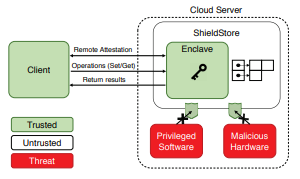
\includegraphics[width=0.6\linewidth]{shieldStoreArchitecture}}
	\caption{Design of ShieldStore}
	\label{fig:shieldStoreArchitecture}
\end{figure}

Its design starts by remote attesting the server-side, verifying \gls{sgx} support of the processor, the code, and other critical memory states of an enclave. By using Intel-\gls{sgx} libraries, the client and the server exchange keys so that a secure channel between both parties is created. The client then sends a request, to which the server deciphers and verifies, accessing the Key-Value Store for the desired data. The server decrypts the stored data and encrypts it again with the session key previously decided when establishing the secure channel with the client. Finally, a reply is sent to the client.    
This design shown in Figure \ref{fig:shieldStoreArchitecture} minimizes the unnecessary memory encryption overhead of paging, and also eliminates \gls{epc} page faults, which are the main factors impacting the performance \gls{sgx}-enabled systems. Adding to the optimization of the index structures, that enabled them for fast access and protection of keys and values, ShieldStore proved to be an efficient and reliable Key-Value store capable of taking the best advantages of \gls{sgx}.\newline

%-----------------------------------------

EnclaveDB \cite{enclavedbPaper} is also an SGX-enabled approach designed to deal also with the protection of data, both when stored and queried. It offers confidentiality and integrity by working alongside Intel-\gls{sgx} in order to handle all the sensitive data (queries, tables, indexes) inside enclave memory, thus keeping the data safe in cases  where the database administrator is malicious, when the \gls{os} or hypervisor is compromised, or even when running the database in an untrusted host.

\begin{figure}[htbp]
	\centering
	{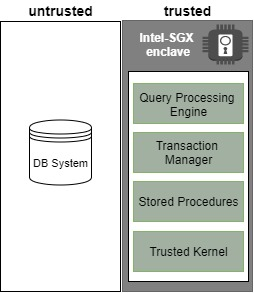
\includegraphics[width=0.3\linewidth]{enclaveDB}}
	\caption{Overview of EnclaveDB compartments}
	\label{fig:enclaveDB}
\end{figure}
 
EnclaveDB is divided into two modules (Figure \ref{fig:enclaveDB}): trusted, running inside the enclave, and untrusted, outside the enclave. The trusted compartment hosts a query processing engine, a transaction manager, pre-compiled stored procedures, and a trusted kernel responsible for sealing and remote attestation. As for the untrusted module, it is responsible to run all the other components of the database system. 
This approach fundamentally provides a database system with a SQL interface capable of ensuring security guarantees, while dealing with low overheads. Also, by depending on a smaller \gls{tcb} than any other conventional database server, the security provided increases considerably, making EnclaveDB a valid approach to work as a trusted database system.

VeritasDB \cite{veritasDB} is a \gls{kvs} that guarantees integrity to the client in the presence of exploits or implementation bugs in the database server. In this approach, the protection enabled by \gls{sgx} is not focused on the \gls{kvs} service itself, but in the protection of the intermediation between clients and \gls{kvs} operations. VeritasDB is implemented as a network proxy that mediates communication between the unmodified clients and the unmodified database server, which can be any off-the-shelf database engine (e.g. Redis, RocksDB, or other solutions). Since the proxy is trusted, the solution addresses security primitives supported in Intel-SGX enclaves, to protect the proxy’s code and state, thus completely eliminating trust in the cloud provider. To perform integrity checks in the proxy, the VeritasDB includes an authenticated Merkle B-tree that leverages features of \gls{sgx} (protected memory, direct access to unprotected memory from enclave code, and \gls{cpu} parallelism) to implement several novel optimizations based on caching, concurrency, and compression.

SPEICHER \cite{speicher} was another approach designed as a secure storage system that not only provides strong confidentiality and integrity properties but also ensures data freshness to protect against rollback/forking attacks. SPEICHER exports a Key-Value (KV) interface backed by Log-Structured Merge Tree (LSM). The solution provides secure data storage and trustable query operations. SPEICHER enforces the security properties on an untrusted host by leveraging shielded execution based on a hardware-assisted \gls{tee} — more specifically, Intel-SGX. The design of SPEICHER extends the trust in shielded execution beyond the secure enclave memory region to ensure that the security properties are also preserved in the stateful setting of an untrusted storage medium. To achieve these security properties while overcoming the architectural limitations of Intel-SGX, the authors designed a direct I/O library for shielded execution, a trusted monotonic counter, a secure LSM data structure, and associated algorithms for storage operations. The SPEICHER prototype is based on the base RocksDB \cite{rocksDB} \gls{kvs} and evaluated using a RocksDB benchmark suite called db\_bench \cite{dbBench}

Finally, we thought it was important to mention again HardIDX since it is an approach to search for ranges and values over encrypted data using hardware support, making it deployable as a secure index in an encrypted database. The approach joins a security proof explicitly including side channels and the protection of the secure index by leveraging Intel-SGX. In a more focused vision,  HardIDX is deployable as a highly performant encrypted database index optimized to require only a few milliseconds for complex searches on large data and scale to almost arbitrarily large indices. The authors argue that the solution only leaks access patterns with the trusted code protected by \gls{sgx} hardware being very small.



\section{Summary and Discussion}
\label{sec:summary}


After going through all those approaches, we can look at the technologies presented in this chapter and pick the ones that we think to suit better our objective for this thesis. 

Starting with \gls{os} isolation systems discussed in \ref{sec:protect_untrustOS}, although capable of assuring a good sense of privacy from the \gls{os}/hypervisor, they do not take into account the potential hardware vulnerabilities that a system can have while making use of sensitive data. 
With that in mind, opting for a \gls{tee} approach made more sense for offering a more complete sense of security.
While \gls{tpm}s have proven to have problems adapting to the Cloud, modern \gls{tee} technology, on the other hand, has proven to be the way to go, by combining hardware solutions with specific software.

Going deeper into these modern technologies in section \ref{sec:hardwareTEEs}, we knew beforehand that our focus would be on Intel-\gls{sgx}. However, we picked it from the two most used (along with ARM TrustZone) mainly due to the fact that ARM TZ supports only one secured zone, which led it to be more adopted by the phone industry, and it is not what we are focusing in this dissertation. On the other hand, Intel-\gls{sgx} is able to support multiple secured zones (enclaves) for each processor, which is really relevant in cloud systems due to the need to manage data from multiple users at once.
Also by not requiring additional code to grant hardware attestation, since its design supports it, Intel-\gls{sgx} is able to keep a smaller \gls{tcb} than ARM TrustZone.

Since the adoption of \gls{tee} technologies was found to drop significantly the overall performance of systems when used by itself, in \ref{sec:sgxFrameworks} we go into detail on how different existing technologies can positively impact the work of \gls{sgx}. Since our focus resides on running applications in this kind of security environment, we found SCONE [\ref{ssec:scone}] to be a good fit. By running containers on top of \gls{sgx} with access to a small library of restricted and secured system calls, this solution has proven to improve significantly the performance of some applications running on top of \gls{sgx}, while still allowing to obtain integrity and confidentiality for the data, as well as other valuable characteristics such as scalability and ease of deployment, which can come in handy when testing our prototype. 









